\section{System Outline}
\label{sec:outline}
\graphicspath{{_Intro/Figures/}}

The communication system under the VLC model operates under the hybrid wireless model paradigm using the VLC channel as the high capacity downlink and another medium for the uplink. This seems to be the accepted model and a reasonable assumption \cite{rah11a}.  \figurename{ \ref{fig:VLCdownBD}} illustrates a block diagram for a typical VLC downlink. 

\subsection{Data Source}
\label{subsec:outlineSource}
The source is an entity that, while performing its tasks, produces information that needs to be communicated to another entity.

\subsection{Coder}
\label{subsec:outlineCoder}
The coder converts data from the source to a binary bit sequence. In this process, it may introduce redudancy to reduce the effect of noise and interference in the channel. 

\subsection{Illumination State}
\label{subsec:outlineIllumination}
The illumination state sets the average output flux and the SPD to be produced by each luminaire. This is a result of a number of factors such as (a) requested illumination level by person in the space (b) optimal energy usage (c) output of 'smart' applications such as circadian control, etc...

\begin{figure}[!t]
	\centering
		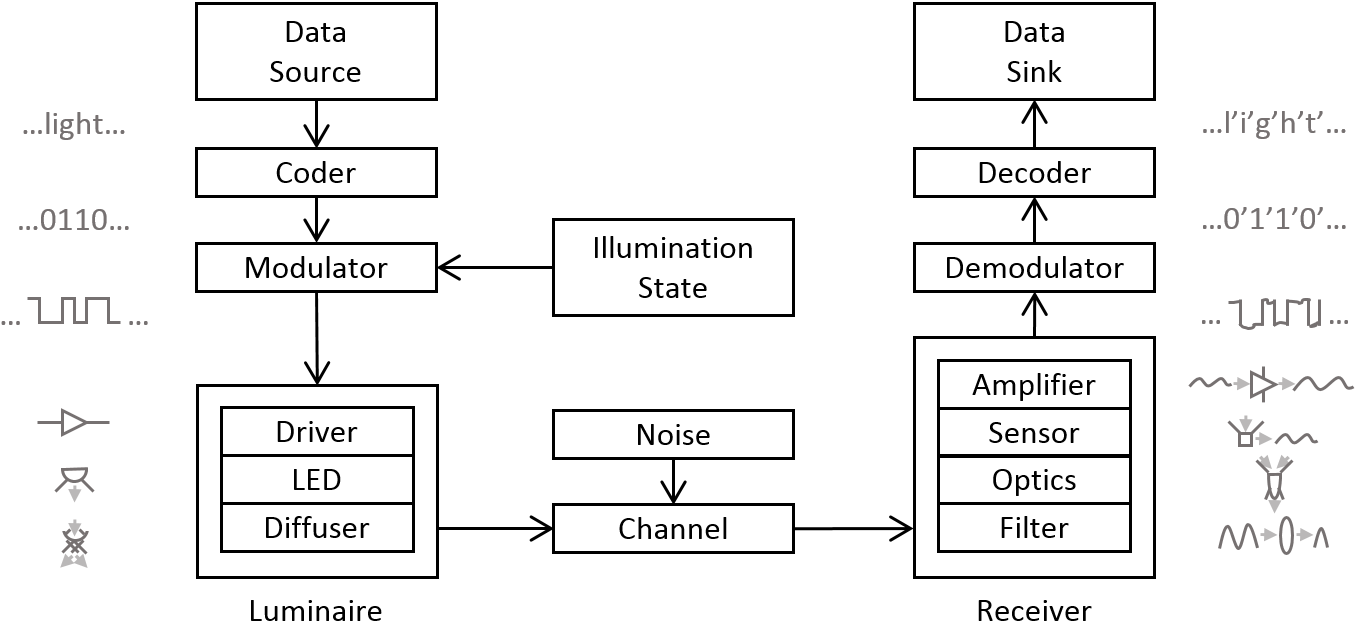
\includegraphics[width=6in]{vlcdownlinkBD.png}
	\caption{VLC downlink block diagram}
	\label{fig:VLCdownBD}
\end{figure}

\subsection{Modulator}
\label{subsec:outlineModulator}
The modulator, with the knowledge of requested flux, converts the bit sequence into a corresponding waveform that drives the luminaire. The frequency of visible light is in the range of about 400-800 THz. The current state-of-art electronics cannot sample and process signals at that high speeds. Thus traditional modulation schemes which vary the amplitude, frequency or phase of the waveforms withinin the RF spectrum cannot be directly implemented within the visible spectrum. Instead, the average power (a.k.a flux/intensity) of the visible waveforms are modulated to transmit data. Optical sensors like PDs produce output current proportional to the intensity of the incident radiation and not the waveform of the radiation itself. This signalling scheme is known as IM/DD. 

\subsection{Luminaire}
\label{subsec:outlineLuminaire}
The luminaire is composed of driver, LED(s) and diffuser. A simple LED driver is a transconductance amplifier whose input is the waveform produced by the modulator. The corresponding output current drives the LED which in turn generates light. 

A luminaire is made up of number of phosphor converted white LEDs or different narrow-band devices which produce diferent colors. A phosphor converted white LED is made by coating a blue LED with yellow phosphor. The blue light excites the yellow phosphor and together they produce white light. 

The diffuser scatters the light produced by the LED(s) to mix the different colors. It also makes the luminous surface appear softer and more pleasing to the eye. Different diffuser front ends generate different sizes of cones of emission. The most common emission pattern is the lambertian pattern. Let $\phi$ be the angle subtended between the transmitter surface normal and direction of emission, $\phi_{1/2}$ be the transmitter semi-angle and $m$ be the order of emission. Then Eq.\ref{eqLambertian} defines the lambertian radiant intensity at any angle $\phi$.

\begin{subequations}
	\begin{gather}
	L(\phi) = \twopartdef{{\frac{(m+1)}{2\pi}}cos^{m}(\phi)}{-\pi/2\leq\phi\leq\pi/2}{0}{\mbox{ else}} \label{eqLambertian} \\
	m = -\frac{\text{ln}(2)}{\text{cos}(\phi_{1/2})} \label{eqLambOrder}
	\end{gather}
\end{subequations}

\subsection{Channel}
\label{subsec:outlineChannel}
The channel is the medium through which information flows. It is made up of all the paths travelled by the light rays between the luminaire and the receiver. Depending on the number of transmitters, colors or number of receiving elements, the channel can be configured into a various single/multiple input single/multiple output configurations.

\subsection{Receiver}
\label{subsec:outlineReceiver}
A receiver is made up of an optical filter, optics, an optical sensor like PD (PIN or APD) and a TIA. Some high speed systems transmit data over a small range of wavelengths (ex Blue (400-500nm)) while the entire visible spectrum is used for illumination. In such cases, a blue filter is used to remove noise from parts of the optical spectrum that do not carry any data. For WDM systems where data is transmitted independently over different parts of the spectrum, multiple non-overlapping filters are used to decorrelate the different streams of information. For single pixel receivers, concentrator optics are used to increase the effective area of the sensor while keeping its capacitance at a minimum. A number of single pixel receivers can be configured in a matrix pattern to realize a non-imaging multiple element receiver. For imaging receivers, imaging optics are used to help decorrelate the multiple channels. Noise introduced by the channel distorts the signal waveform. 

\subsection{Demodulator}
\label{subsec:outlineDemodulator}
The demodulator, with prior knowledge of the modulation scheme implemented, tries recreate the transmitted bit sequence from the received waveform. Significant noise that is not orthogonal to the signal waveform can introduce errors in the demodulated sequence.

\subsection{Decoder}
\label{subsec:outlineDecoder}
The decoder, with prior knowledge of the coding scheme implemented, tries to recover the transmitted data from the bit stream. Redundancy itroduced in the coded data can help the decoder to detect and rectify errors.

\subsection{Data Sink}
\label{subsec:outlineSink}
Ideally, the data sink is the entity to which the information was transmitted to. 
